\section{Preliminary Results}
We present some preliminary results on multi-object trajectory inference.
There are two experiments. In the first experiment, we seek to understand
the speed distributions of individuals and whether the distributions can be
characterized into different movement types such as walking, biking and
riding in a vehicle. In the second experiment, we evaluate our inference
algorithm on a number of synthetic data sets generated from pre-determined
movement types.

\subsection{Speed Distributions}
We asked 10 students to record their GPS traces for a full day
using a tool called GPSlogger which logs the location and speed 
at 10-second intervals. Each student may exhibit several travel patterns
on that day, e.g., walking, biking, or riding the campus shuttle bus.
We collected the traces, chopped them into segments according to time and then
cluster the traces according to their speed distributions. We find distinct
clusters which correspond to walking and biking, respectively. 
Example speed distributions of some individuals are shown 
in Figure~\ref{fig:dist}. 

\begin{figure}
\begin{minipage}[th]{0.48\columnwidth}
\centering
\includegraphics[scale=0.25]{ed_walk.eps}
{\small(a) Walking}

\end{minipage}
\begin{minipage}[th]{0.48\columnwidth}
\centering
\includegraphics[scale=0.25]{bike_youer.eps}
{\small(b) Biking}
\end{minipage}
\caption{Example Speed Distributions}
\label{fig:dist}
\end{figure}

%\KZ{Show a fig of three speed distributions (histograms) for these three modes.}

\subsection{Trajectory Inference}
We synthesize three datasets on the map of a university campus. Each
dataset contains the moving trajectories of a number of users and 
is generated as follows.

\noindent(1) Randomly select the start and end locations on 
the map for each user;\\ 
(2) For each user, randomly determine if he or she is walking,
biking or driving and randomly generate a trajectory according to the 
corresponding speed distribution we recorded earlier;\\
(3) Induce contact records from these trajectories.

The three datasets differ by the size of the map, the number of
users on the map and thus the number of contact records. 
A fragment of one generated trajectory looks like this:
\begin{center}
\small
\begin{tabular}{ c | c | c | c  }

  Road Id & Relative location & Speed & Time \\ \hline
2	&2.80	& 2.0	& 0.0 \\
2	&2.12	&1.37	&0.5\\
2	&1.02	&2.19 	&1.0\\
\dots &\dots  & \dots  & \dots  \\
1	&26.82	&6.45 &	87.0\\
1	&25.28 	&3.07 	&87.5\\
1	&24.67	&1.23 	&88.0\\
\end{tabular}
\end{center}
Each road is a 1-D array. The relative location in the table is the distance relative to the left-most point of the corresponding road.
%\KZ{No need to have so many decimal places in the above table.
%Also explain what it means by relative locations?}

The trajectories in the datasets serve as the ground truth, while the
most likely trajectories (in the form of a sequence of exact locations 
for each contact point) infered by our algorithm are compared against the
ground truth.

%In the following subsections, we first introduce the data set, then
%compare the accuracy of our approach with the backgroud truth data set.
%\subsection{Data Set}
%We use synthetic data sets. Each set was generated using the following rules.
%The number of targets, map size and simulation time are all parameters to input. The data set will contain two parts. GPS records and contact records. 
%
%\end{center}
%A contact record may looks like:
%\begin{center}
%\begin{tabular}{ c|c|c}
%
%Id1 & Id2 & Time \\ \hline
%0 &2 & 2.0 \\
%0 &2 & 2.5 \\
%0 &2 & 3.0 \\
%\dots & \dots & \dots \\
%0 & 1 & 72.5 \\
%0 & 3 & 73.0 \\
%
%\end{tabular}
%
%\end{center}
%
%We prepared three data sets with different scales.
%\begin{center}
%
%\begin{tabular}{ p{1cm} | p{1cm} | p{1.5cm} | p{1.5cm} | p{1.5cm} | p{1.5cm}}
%Data set Id & Map size & Number of people & Duration (seconds) & Number of contacts \\ 
%\hline
%1 & 450  & 5 & 90 & 46 \\
%2 & 860  & 15 & 90 & 73 \\
%\dots & \dots   & \dots& \dots& \dots \\
%\end{tabular}
%\end{center}
%\subsection{Accuracy}
%We compared the inference result with the ground-truth GPS records. 

Figure~\ref{fig:qande}(a) shows the inference error (in terms of distance
in meters to the ground truth path) for a small dataset of 16 users 
on a map with total road length of 860 meters. 
%\KZ{What is the exact definition of this error and the map size?} 
In real world applications, 
contacts can be detected within radio sight, say 8 meters for bluetooth
communication. If we ignore errors smaller than that range, 
the precision of our inference algorithm goes up to over 80\%
on average, which is shown in Figure~\ref{fig:qande}(b).
The inference precision of the other two data sets is recorded at 
81\% and 90\%, respectively. 
%\KZ{We need a number here: precision for all three datasets. Also
%how did we calculate this precision, give the formula.}

\begin{figure}
\begin{minipage}[th]{0.48\columnwidth}
\centering
\includegraphics[scale=0.25]{error.eps}
{\small(a)}

\end{minipage}
\begin{minipage}[th]{0.48\columnwidth}
\centering
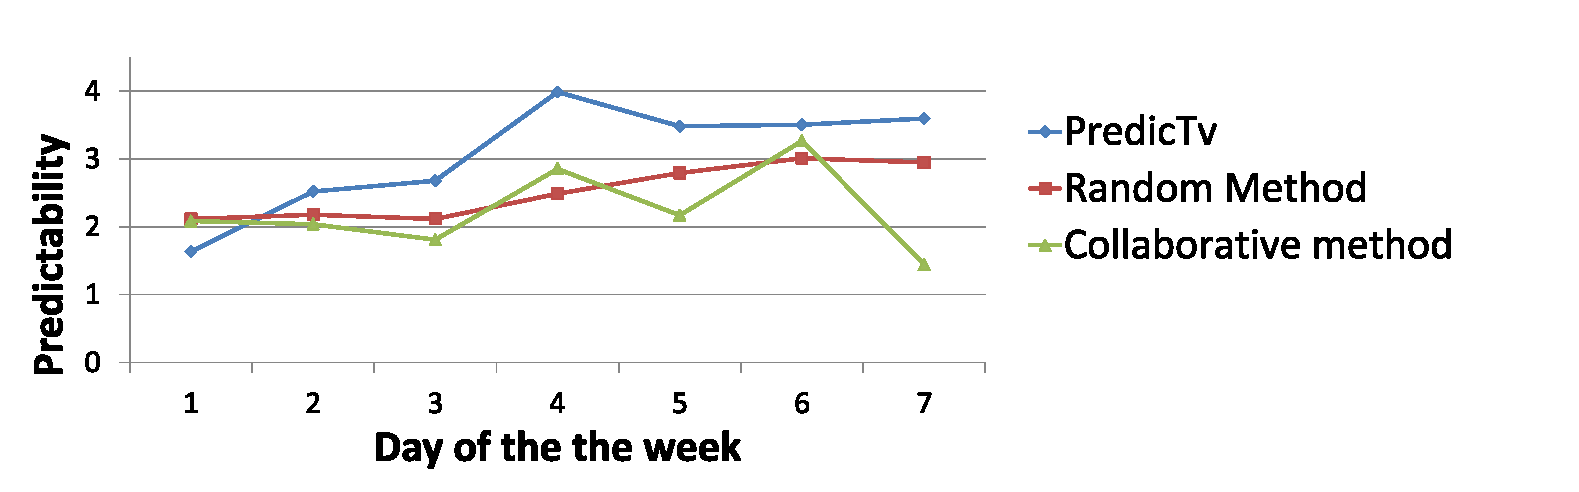
\includegraphics[scale=0.25]{precision.eps}
{\small(b)}
\end{minipage}
\caption{(a) Inference Error (meters). 
(b) Inference Precision (with tolerance).}
\label{fig:qande}
\end{figure}




